%% Appendix B — Supplementary ML material: grid search figure, synthetic-trace model, CNN
\section{Supplementary ML Material}
\label{appendix:ml}

This appendix collects the full architecture-search figure of
Section~\ref{subsec:arch_search} and the core code behind the raw-trace study of
Section~\ref{subsec:cnn} together with the figures it produces.  The synthetic
generator and the \texttt{ReadoutCNN} are reproduced below in condensed form,
omitting data loading, calibration of the per-sample noise covariances, and
plotting; the full \texttt{SSRO\_synthetic\_CNN.ipynb} notebook is in the same
repository as the listings of Appendix~\ref{appendix:code}.

\begin{figure}[ht]
  \centering
  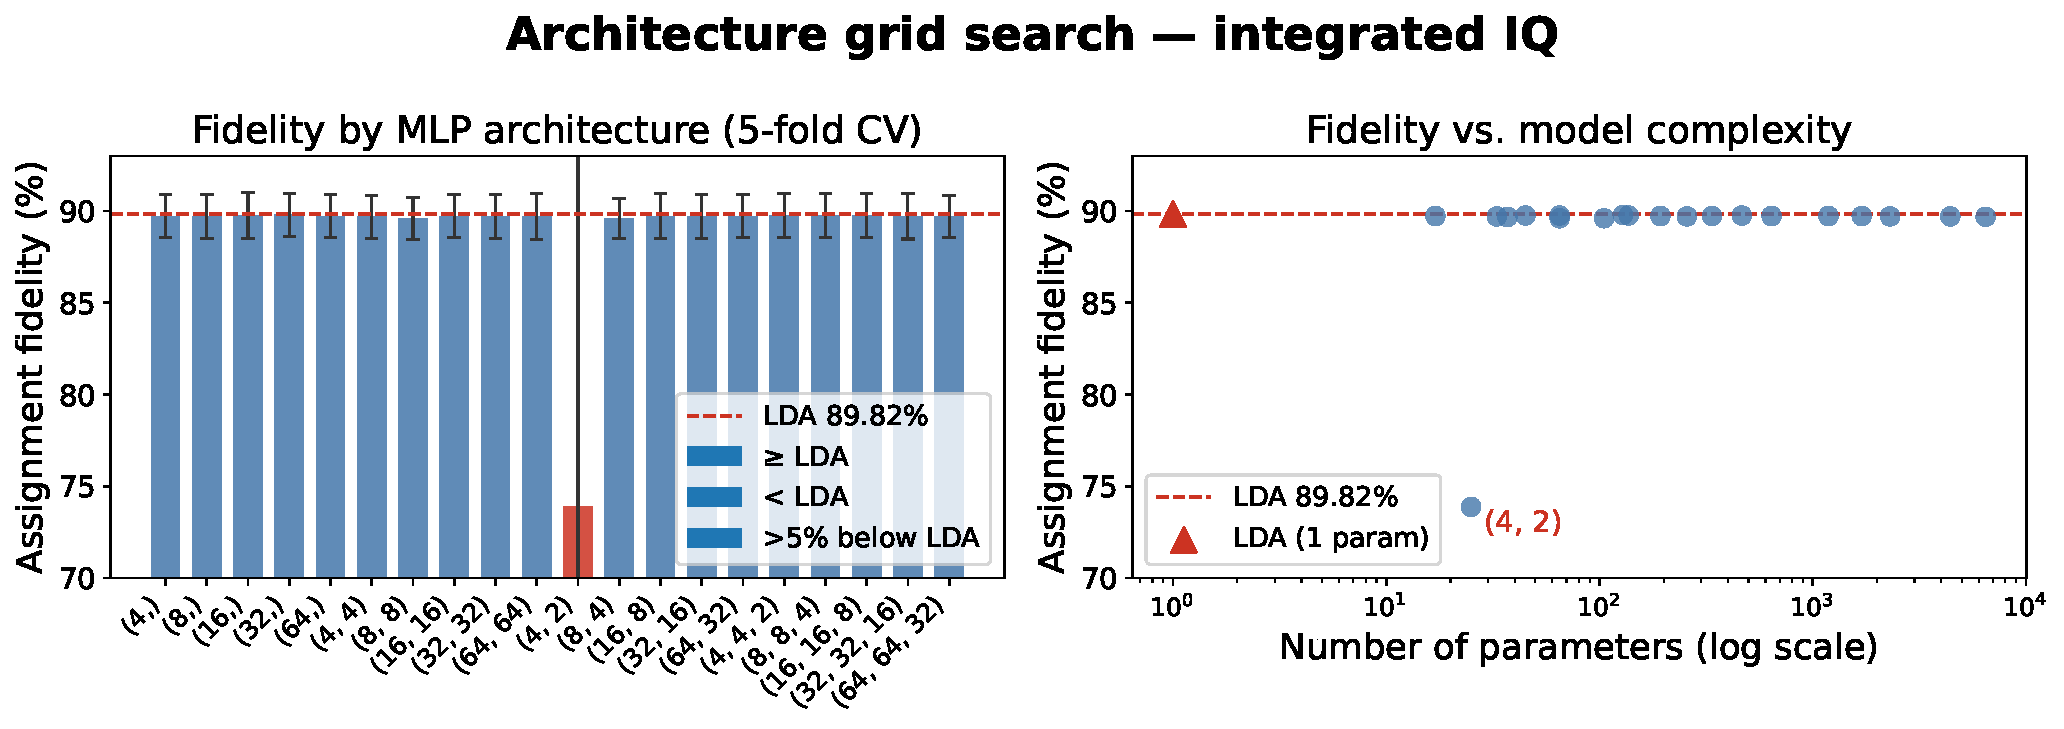
\includegraphics[width=0.95\columnwidth]{code/figures/fig5_grid_search}
  \caption{Architecture grid search results on integrated IQ data (5-fold
    CV), the full version of Table~\ref{tab:arch_search}.  \emph{Left}:
    assignment fidelity per MLP architecture; the red
    dashed line is the LDA baseline (89.82\%).  All architectures except the
    degenerate (4,\,2) configuration lie within CV noise of LDA.  \emph{Right}:
    fidelity vs.\ parameter count on a log scale.  No trend with model size
    is visible across three orders of magnitude.  The one outlier, the (4,\,2)
    architecture (a 4-neuron layer feeding a 2-neuron layer), sits at
    $\approx\!74\%$ with a large cross-validation spread ($\pm 0.20$): the
    two-neuron bottleneck trains unstably, collapsing on some folds rather than
    failing for lack of capacity.  It is excluded from Table~\ref{tab:arch_search}.}
  \label{fig:grid_search}
\end{figure}

\subsection{Synthetic Trace Generator}
\label{appendix:gen_traces}

Each shot is a noisy cavity response sampled over $T$ points.  For $\ket{1}$
shots, the signal switches from $\boldsymbol{\mu}_1$ to $\boldsymbol{\mu}_0$ at a
relaxation sample $t^*$ drawn from a geometric distribution with per-sample rate
$1 - e^{-1/T_1}$ (the discrete-time analogue of exponential $T_1$ decay).

\begin{minted}[fontsize=\small,linenos,breaklines]{python}
def generate_traces(state, N, T, signal0, signal1, cov0_ps, cov1_ps,
                    T1_samples, rng):
    """Generate N synthetic raw IQ traces (N, T, 2) for a prepared state.
    |1> shots may relax at sample t* ~ Geometric(1 - exp(-1/T1))."""
    L0 = np.linalg.cholesky(cov0_ps)
    L1 = np.linalg.cholesky(cov1_ps)
    z  = rng.standard_normal((N, T, 2)).astype(np.float32)
    relax_times = np.full(N, -1, dtype=int)

    if state == 0:                       # |0>: constant state, no relaxation
        traces = signal0[None, :, :] + z @ L0.T.astype(np.float32)
    else:                                # |1>: may decay to |0> at t*
        p = 1.0 - np.exp(-1.0 / T1_samples)
        u = rng.uniform(0, 1, N)
        t_star = np.floor(np.log(u) / np.log(1 - p)).astype(int)
        relaxes = t_star < T
        relax_times[relaxes] = t_star[relaxes]
        sig = np.tile(signal1[None, :, :], (N, 1, 1)).copy()
        for i in np.where(relaxes)[0]:
            sig[i, t_star[i]:, :] = signal0[t_star[i]:, :]
        traces = sig + z @ L1.T.astype(np.float32)
    return traces, relax_times
\end{minted}

\subsection{\texttt{ReadoutCNN} and Training}
\label{appendix:cnn_code}

\begin{minted}[fontsize=\small,linenos,breaklines]{python}
class ReadoutCNN(nn.Module):
    """1D CNN on raw IQ traces. Input (batch, T, 2) -> logit for P(|1>).
    953 params; hls4ml/ZCU216 target, ap_fixed<16,6>, ~100-200 ns @ 250 MHz."""
    def __init__(self):
        super().__init__()
        self.conv = nn.Sequential(
            nn.Conv1d(2, 8,  kernel_size=8, stride=2, padding=3), nn.ReLU(),
            nn.Conv1d(8, 16, kernel_size=4, stride=2, padding=1), nn.ReLU(),
        )
        self.head = nn.Sequential(
            nn.AdaptiveAvgPool1d(1), nn.Flatten(),
            nn.Linear(16, 16), nn.ReLU(), nn.Linear(16, 1),
        )
    def forward(self, x):                # (batch, T, 2) -> (batch, 2, T)
        return self.head(self.conv(x.permute(0, 2, 1)))

model     = ReadoutCNN().to(device)
optimizer = torch.optim.Adam(model.parameters(), lr=1e-3)
scheduler = torch.optim.lr_scheduler.CosineAnnealingLR(optimizer, T_max=EPOCHS)
loss_fn   = nn.BCEWithLogitsLoss()       # EPOCHS = 60, batch size 256

for epoch in range(EPOCHS):
    model.train()
    for xb, yb in dl_train:
        xb, yb = xb.to(device), yb.to(device)
        loss = loss_fn(model(xb), yb)
        optimizer.zero_grad(); loss.backward(); optimizer.step()
    scheduler.step()
\end{minted}

\subsection{Supplementary Figures}
\label{appendix:supp_figures}

\begin{figure}[ht]
  \centering
  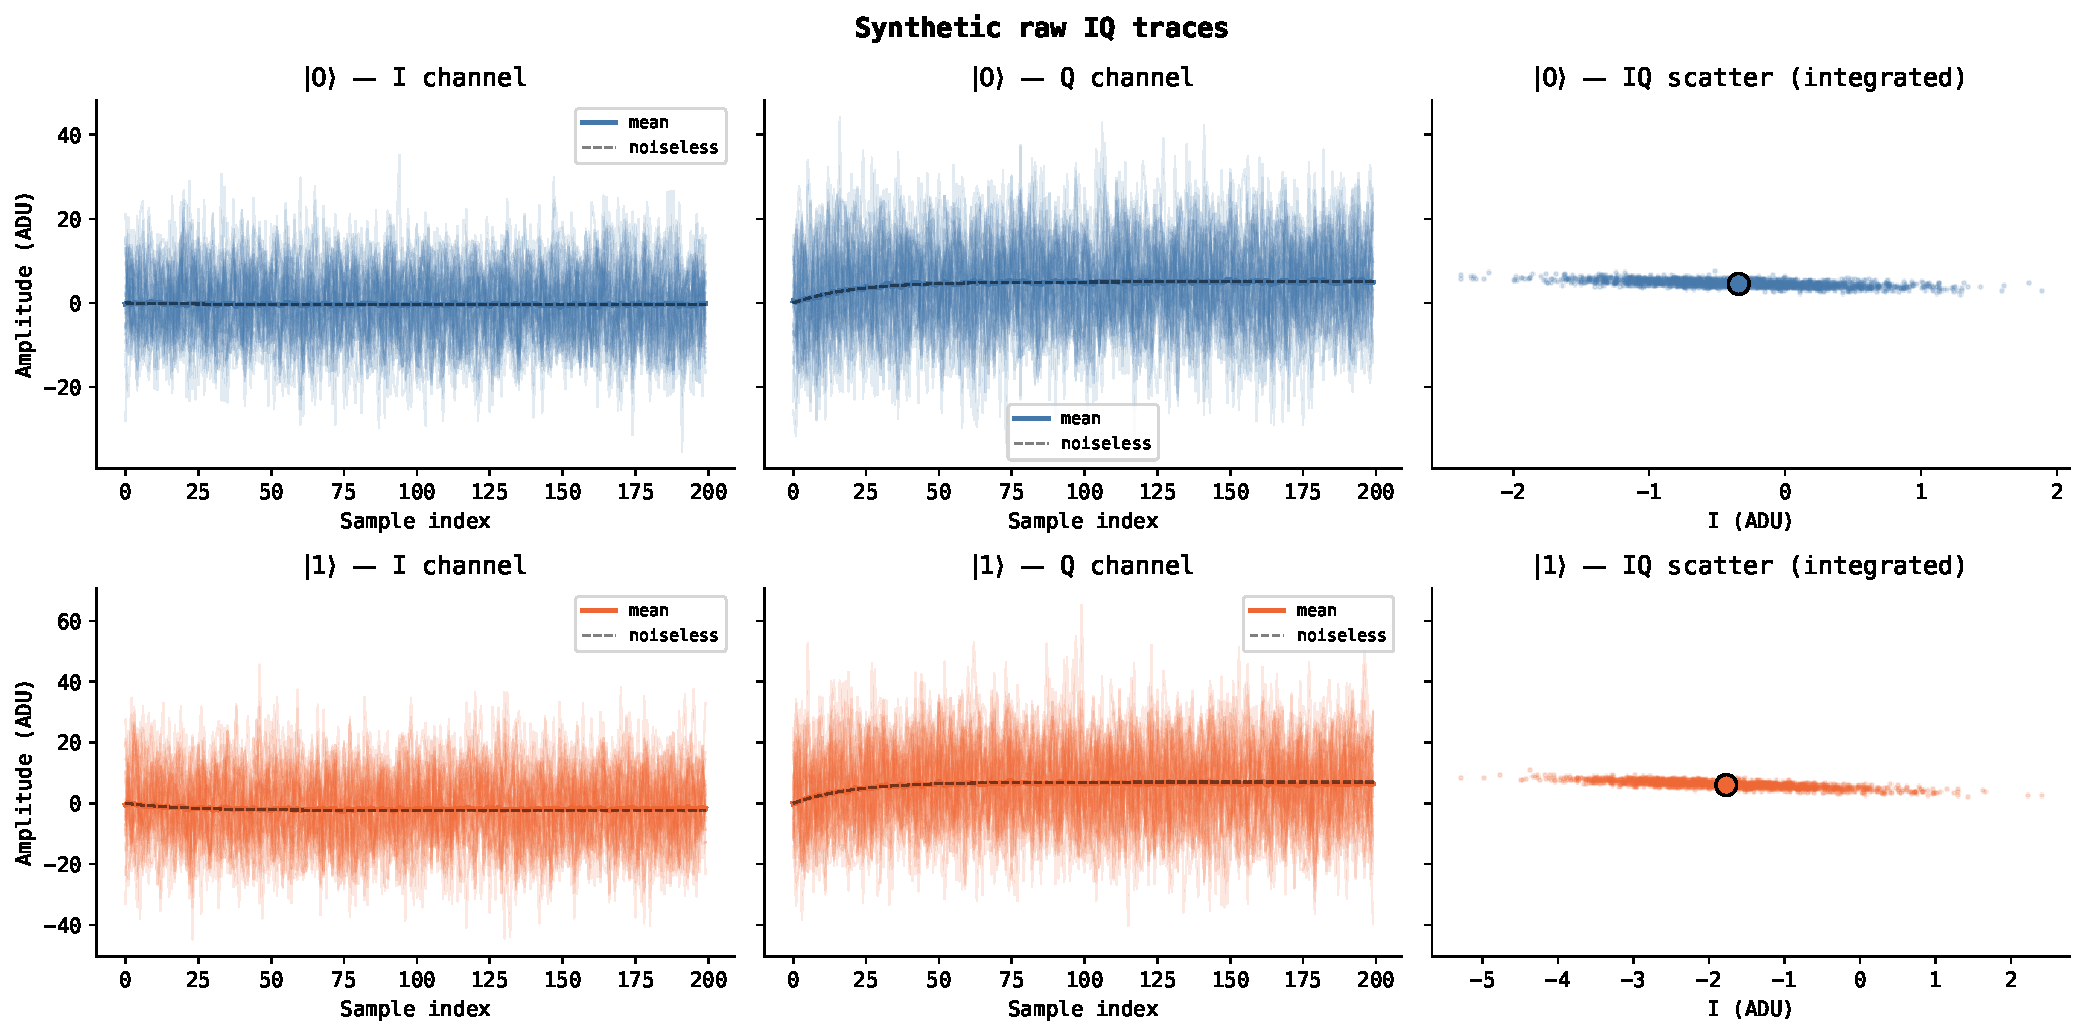
\includegraphics[width=0.92\columnwidth]{code/figures/synthetic_traces}
  \caption{Synthetic raw IQ traces generated by
    Listing~\ref{appendix:gen_traces}'s model and used in
    Section~\ref{subsec:cnn}.  Each time-trace panel overlays 30 noisy shots
    (faint) with the shot-averaged mean (solid) and the noiseless cavity-ring-up
    envelope (dashed).  \emph{Top row}: $\ket{0}$
    shots; both quadratures ring up and plateau near the $\ket{0}$ centroid.
    \emph{Bottom row}: $\ket{1}$ shots; the Q channel plateaus at the $\ket{1}$
    centroid.  \emph{Right column}: integrated IQ scatter after rectangular
    averaging; the $\ket{1}$ cloud is broader, consistent with the covariance
    asymmetry in Table~\ref{tab:iq_stats}.  The traces are generated directly in
    the IQ frame of Figure~\ref{fig:iq_scatter}, so the integrated clouds compare
    with Table~\ref{tab:iq_stats} without any rotation (the self-consistency check
    of Section~\ref{subsec:cnn}).}
  \label{fig:supp_traces}
\end{figure}

\begin{figure}[ht]
  \centering
  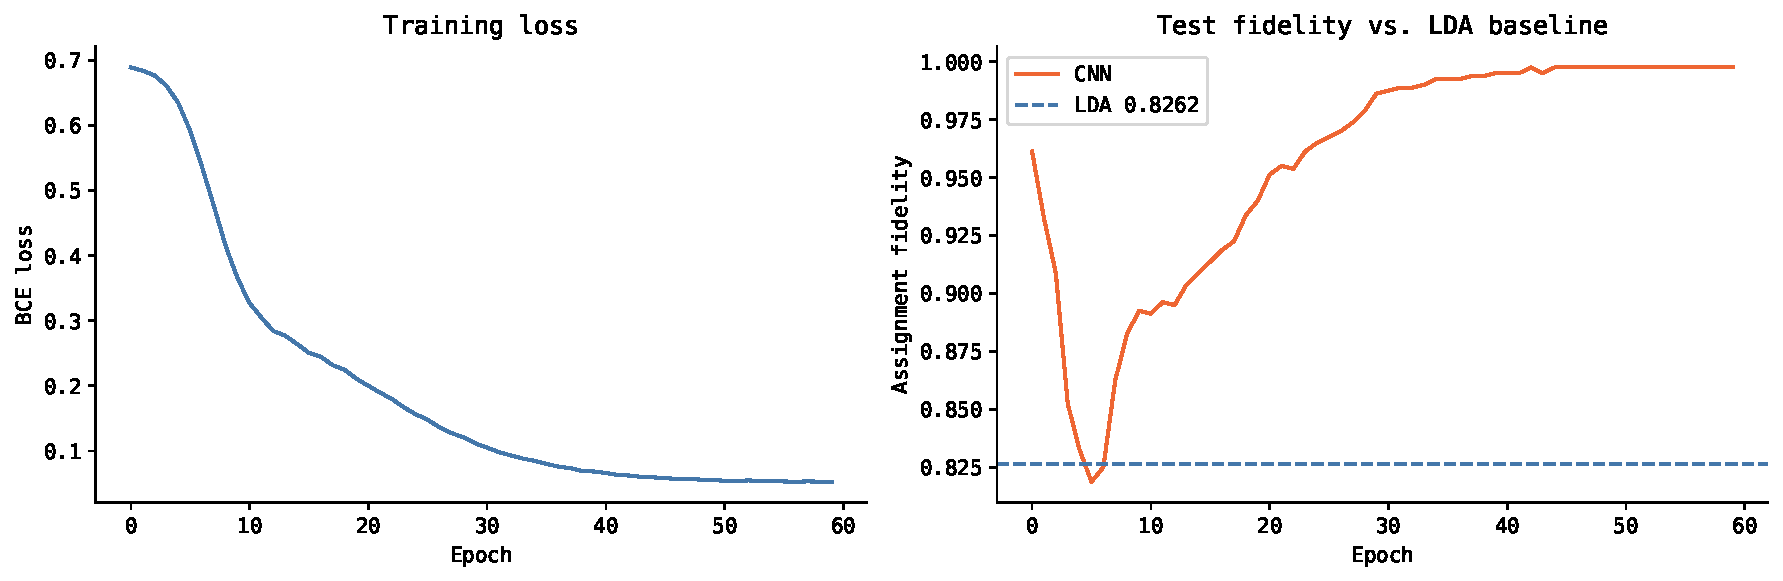
\includegraphics[width=0.85\columnwidth]{code/figures/training_curve}
  \caption{CNN training curves over the 60 training epochs.  \emph{Left}: binary
    cross-entropy loss on the
    training set, converging smoothly within about 40 epochs.  \emph{Right}:
    test-set assignment fidelity per epoch, reaching $\approx\!99.75\%$ and
    remaining well above the LDA baseline on the synthetic data ($0.826$,
    dashed).  The absence of overfitting is consistent with the small model
    size (953 parameters).}
  \label{fig:supp_training}
\end{figure}

\begin{figure}[ht]
  \centering
  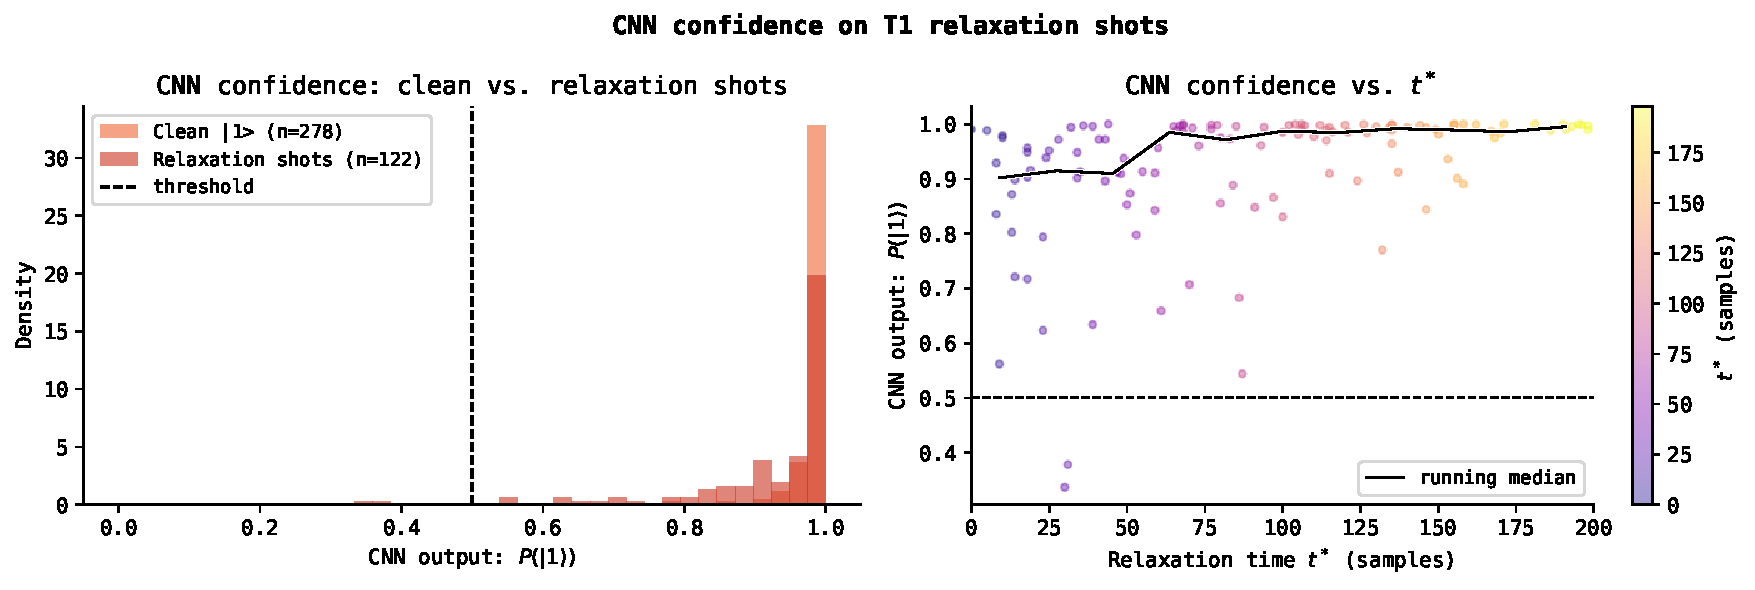
\includegraphics[width=\columnwidth]{code/figures/cnn_relaxation_confidence}
  \caption{CNN confidence on $T_1$-relaxation shots, the mechanism behind the
    recovery reported in Section~\ref{subsec:cnn}.  All quantities are evaluated
    on the $\ket{1}$ shots of the held-out test set only.  \emph{Left}:
    distribution of
    the CNN output $P(\ket{1})$ for clean $\ket{1}$ shots (orange, $n=278$) versus
    shots
    that relaxed within the window (red, $n=122$); the relaxation shots spread
    toward the
    decision threshold.  \emph{Right}: $P(\ket{1})$ versus relaxation time $t^*$,
    coloured by $t^*$, with a running median.  Shots that relax late (most of the
    trace in $\ket{1}$) are classified with near-certainty, while shots that relax
    early are correctly driven toward ambiguity.  LDA, which sees only the
    integrated mean, cannot make this distinction.}
  \label{fig:cnn_confidence}
\end{figure}
